\section{Erzeugung von LALR-Parsern mit \textsl{Bison}}
Die von dem Parser-Generator \textsl{Bison} erzeugten Parser sind LALR-Parser.
\textsl{Bison} bietet die M\"oglichkeit, die erzeugten Mengen von e.m.R.s textuell oder
grafisch darzustellen.  Abbildung \ref{fig:cc.y} zeigt, wie die Grammatik aus Abbildung
\ref{fig:dragon-book.grammar} als Eingabe-Datei f\"ur \textsl{Bison} formatiert werden kann.
Da es uns hier nur um die Erzeugung der Zustands-Mengen geht, enth\"alt die Datei weder
Deklarationen, die zur Anbindung eines Scanners erfoderlich w\"aren, noch semantische Aktionen.

\begin{figure}[!ht]
\centering
\begin{Verbatim}[ frame         = lines, 
                  framesep      = 0.3cm, 
                  labelposition = bottomline,
                  numbers       = left,
                  numbersep     = -0.2cm,
                  xleftmargin   = 0.8cm,
                  xrightmargin  = 0.8cm,
                ]
    %%
    S : C C;
    
    C : 'x' C
      | 'y'
      ;     
    %%
\end{Verbatim}
\vspace*{-0.3cm}
\caption{Die Grammatik aus Abbildung \ref{fig:dragon-book.grammar} im \textsl{Bison}-Format.}
\label{fig:cc.y}
\end{figure}

\noindent
\"Ubersetzen wir die in Abbildung \ref{fig:cc.y} gezeigte Datei mit dem Befehl
\[ \texttt{bison -v -g cc.y} \]
so werden von \textsl{Bison} zwei Dateien erzeugt:
\begin{enumerate}
\item Die Option ``\texttt{-v}'' (\emph{verbose}) bewirkt, dass die Datei
      \texttt{cc.output} erzeugt wird.  Diese Datei enth\"alt die Zust\"ande des
      LALR-Parsers und wird in Abbildung \ref{fig:cc.output} gezeigt.
\item Die Option ``\texttt{-g}'' (\emph{graphic}) erzeugt die Datei
      \texttt{cc.vcg}.  Die Datei-Endung \texttt{.vcg} steht als Abk\"urzung f\"ur 
      \emph{visualization of compiler graphs}.
      Diese Datei stellt den Goto-Graphen der Grammatik im
      \emph{VCG-Format} dar und l\"asst sich mit Hilfe geeigneter Werkzeuge grafisch
      darstellen.  
      Ein solches Werkzeug ist \texttt{aiSee}, dass Sie im Internet unter der Adresse
      \\[0.2cm]
      \hspace*{1.3cm}
      \texttt{http://www.aisee.com/}
      \\[0.2cm]
      finden.  Dort k\"onnen Sie eine Demoversion kostenlos herunterladen.
\end{enumerate}

\begin{figure}[!ht]
\centering
\begin{Verbatim}[ frame         = lines, 
                  framesep      = 0.3cm, 
                  labelposition = bottomline,
                  numbers       = left,
                  numbersep     = -0.2cm,
                  xleftmargin   = 0.8cm,
                  xrightmargin  = 0.8cm,
                ]
    Grammar
        0 $accept: S $end
        1 S: C C
        2 C: 'x' C
        3  | 'y'
    Terminals, with rules where they appear
    $end (0) 0
    'x' (120) 2
    'y' (121) 3
    error (256)
    Nonterminals, with rules where they appear
    $accept (5)
        on left: 0
    S (6)
        on left: 1, on right: 0
    C (7)
        on left: 2 3, on right: 1 2
    state 0
        0 $accept: . S $end
        'x'  shift, and go to state 1
        'y'  shift, and go to state 2
        S  go to state 3
        C  go to state 4
    state 1
        2 C: 'x' . C
        'x'  shift, and go to state 1
        'y'  shift, and go to state 2
        C  go to state 5
    state 2
        3 C: 'y' .
        $default  reduce using rule 3 (C)
    state 3
        0 $accept: S . $end
        $end  shift, and go to state 6
    state 4
        1 S: C . C
        'x'  shift, and go to state 1
        'y'  shift, and go to state 2
        C  go to state 7
    state 5
        2 C: 'x' C .
        $default  reduce using rule 2 (C)
    state 6
        0 $accept: S $end .
        $default  accept
    state 7
        1 S: C C .
        $default  reduce using rule 1 (S)
\end{Verbatim}
%$
\vspace*{-0.3cm}
\caption{Die Datei \texttt{cc.output}.}
\label{fig:cc.output}
\end{figure} 

Wir diskutieren nun die in Abbildung \ref{fig:cc.output} gezeigte Datei \texttt{cc.output}
Zeile f\"ur Zeile.
\begin{enumerate}
\item Die Zeilen 1 -- 5 zeigen die zu Grunde liegende Grammatik.  Die 0-te Regel hat hier
      die Form
      \\[0.2cm]
      \hspace*{1.3cm}
      $\texttt{\$accept: S \$end}$
      \\[0.2cm]
      und entspricht im wesentlichen unserer Regel
      \\[0.2cm]
      \hspace*{1.3cm}
      $\widehat{S} \rightarrow S$,
      \\[0.2cm]
      wobei der String ``\texttt{\$end}''
      %\$
      f\"ur das Ende der Eingabe steht.  Bei Bison wird also das Datei-Ende-Zeichen
      \textsc{Eof} mit zu der Regel hinzugenommen.

      Wie Sie sehen, sind die einzelnen Grammatik-Regeln mit 0 beginnend numeriert.
      Auf diese Nummerierung wird  Bezug genommen.
\item Die Zeilen 7 -- 10 listen alle Terminale auf, die in der Grammatik verwendet
      werden.  Die Zeile
      \\[-0.2cm]
      \hspace*{1.3cm}
      $\texttt{'x' (120) 2}$
      \\[0.2cm]
      ist beispielsweise wie folgt zu lesen:
      \begin{enumerate}
      \item \texttt{'x'} ist ein Terminal
      \item mit dem \textsc{Ascii}-Code 120 und
      \item dieses Terminal tritt in der Regel 2 auf.
      \end{enumerate}
      Neben den vom Benutzer in der Grammatik definierten Terminalen ``\texttt{x}'' und
      ``\texttt{y}'' f\"uhrt \textsl{Bison} noch die beiden Terminale
      ``\texttt{\symbol{36}end}'' und ``\texttt{error}'' ein.  Ersteres bezeichnet das
      Ende der Eingabe, letzteres steht f\"ur ein Token, dass nicht in der Eingabe-Sprache vorkommt.
\item Die Zeilen 11 -- 17 listen die syntaktischen Variable, die hier als Nicht-Terminale
      bezeichnet werden, auf und geben die Regeln an, wo diese Variablen auftreten.
      Auch den Variablen werden Zahlen zugeordnet.  Diese Zahlen spielen jedoch nur
      in dem Code des von Bison erzeugten Parsers eine Rolle.
\item Der Rest der Datei zeigt die Zust\"ande und spezifiziert gleichzeitig die Funktionen
      $\textsl{goto}()$ und $\textsl{action}()$.  Bei den Zust\"anden wird allerdings nicht
      die gesamte Menge der e.m.R. angegeben, sondern es wird nur eine Menge
      $\textsc{M}^-$ angegeben, aus der sich mit Hilfe der Funktion $\textsl{closure}()$
      die gesamte Menge nach der Formel
      \\[0.2cm]
      \hspace*{1.3cm}
      $\textsc{M} = \textsl{closure}(\textsc{M}^-)$
      \\[0.2cm]
      berechnen l\"asst.  Au{\ss}erdem werden die Mengen der Folge-Token nicht angegeben.
      Wir betrachten nun zwei der Zust\"ande im Detail:
      \begin{enumerate}
      \item Der Zustand ``\texttt{state 1}'', der in der Zeile 25 spezifiziert
            wird, entspricht der Menge
            \\[0.2cm]
            \hspace*{-0.8cm}
            $s_1 = \textsl{closure}(\{ C \rightarrow \quoted{x} \bullet C \})$
            \\[0.1cm]
            Hier ist zu beachten, dass an Stelle des Markierungs-Symbols ``$\bullet$''
            ein Punkt ``\texttt{.}'' verwendet wird.  
            
            In Zeile 26 wird  spezifiziert, dass
            \\[0.2cm]
            \hspace*{1.3cm} 
            $\textsl{goto}(s_1, \squoted{x}) = s_1$ \quad und \quad
            $\textsl{action}(s_1, \squoted{x}) =\langle \texttt{shift}, s_1 \rangle$
            \\[0.2cm]
            gilt.  Analog ist Zeile 27 als
            \\[0.2cm]
            \hspace*{1.3cm} 
            $\textsl{goto}(s_1, \squoted{y}) = s_2$ \quad und \quad
            $\textsl{action}(s_1, \squoted{x}) = \langle \texttt{shift}, s_2 \rangle$
            \\[0.2cm]
            zu lesen und in Zeile 28 haben wir
            \\[0.2cm]
            \hspace*{1.3cm}
            $\textsl{goto}(s_1,C) = s_5$.
      \item Der Zustand ``\texttt{state 2}'', der in der Zeile 30 spezifiziert
            wird, entspricht der Menge
            \\[0.2cm]
            \hspace*{1.3cm}
            $s_2 = \textsl{closure}\bigl(\bigl\{ C \rightarrow \squoted{y} \bullet:  \{
            \squoted{x}, \squoted{y},\symbol{36} \bigr\}\bigr)$.
            \\[0.2cm]
            Zeile 31 ist als
            \\[0.2cm]
            \hspace*{1.3cm}
            $\textsl{action}(s_2,t) = \langle \texttt{reduce}, C \rightarrow \quoted{x} C \rangle$ 
            \quad f\"ur alle Token $t$
            \\[0.2cm]
            zu lesen.
      \end{enumerate}
\end{enumerate}
Neben der eben diskutierten textuellen Darstellung bietet \textsl{Bison} noch die Option, die Zust\"ande des
LALR-Parsers grafisch darzustellen.  Dazu erzeugt \textsl{Bison} zun\"achst die Datei \texttt{cc.vcg}, die dann
beispielsweise mit dem Werkzeug \texttt{aisee} visualsiert werden kann.  Abbildung
\ref{fig:bison-goto-graph.eps} zeigt diese Visualisierung. 

\begin{figure}[!ht]
\centering
      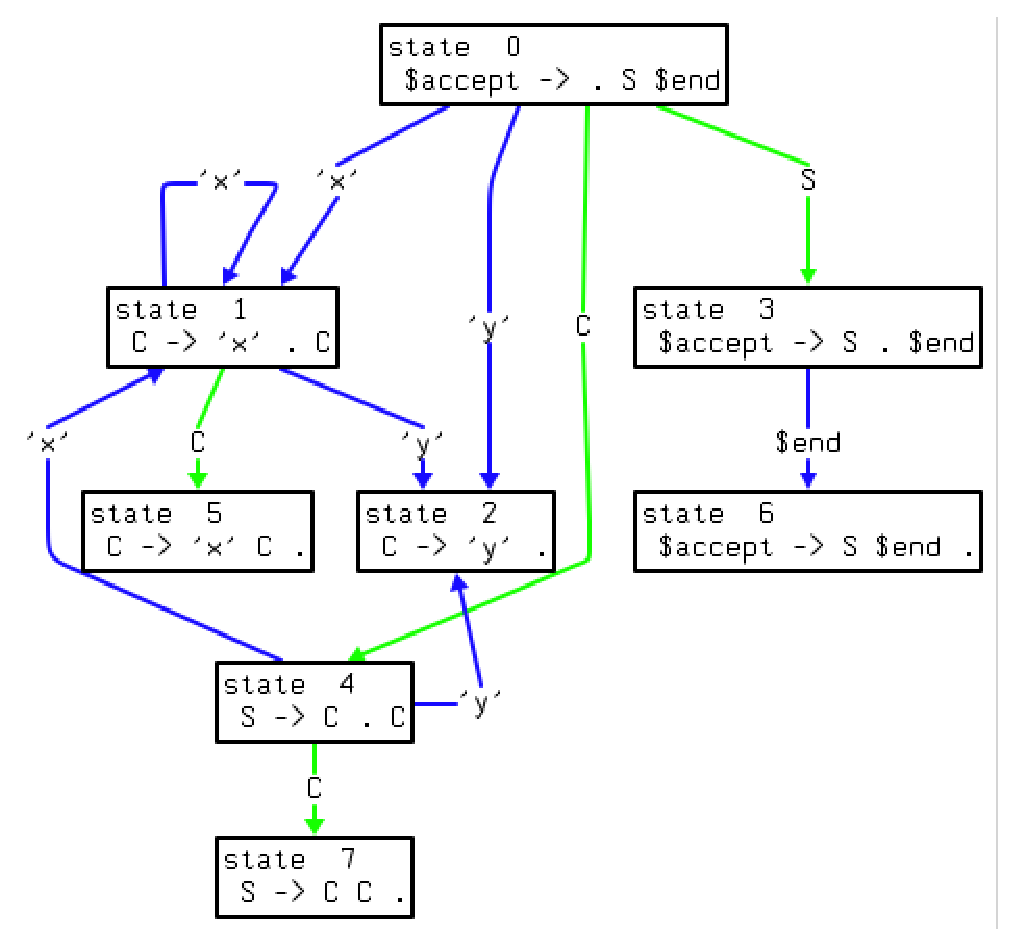
\epsfig{file=Abbildungen/cc-bison, scale=0.5}
  \caption{Von \textsl{Bison} erzeugte grafische Darstellung des Goto-Graphen der Grammatik aus Abbildung \ref{fig:dragon-book.grammar}.}
  \label{fig:bison-goto-graph.eps}
\end{figure}
\pagebreak

\vspace*{\fill}
\pagebreak

\section{Die Behandlung von Konflikten mit \textsl{Bison}}
\textsl{Bison} kann auch dann noch Grammatiken erzeugen, wenn bei der Konstruktion der Zust\"ande Shift-Reduce-
oder Reduce-Reduce-Konflikte auftreten.  Wir besprechen anhand zweier typischer Situationen, wie
\textsl{Bison} in solchen F\"allen vorgeht.

\subsection{Operator-Pr\"azedenzen}
\begin{figure}[!ht]
\centering
\begin{Verbatim}[ frame         = lines, 
                  framesep      = 0.3cm, 
                  labelposition = bottomline,
                  numbers       = left,
                  numbersep     = -0.2cm,
                  xleftmargin   = 0.8cm,
                  xrightmargin  = 0.8cm,
                ]
    %token N
    
    %%
    
    E : E '+' E
      | E '*' E
      | N
      ;
\end{Verbatim}
\vspace*{-0.3cm}
\caption{\textsl{Bison}-Darstellung der Grammatik aus Abbildung \ref{fig:shift-reduce-conflict.grammar}.}
\label{fig:conflict.y}
\end{figure}

\noindent
Wir beginnen mit der in Abbildung \ref{fig:shift-reduce-conflict.grammar} gezeigten Grammatik f\"ur
arithmetische Ausdr\"ucke.  Abbildung \ref{fig:conflict.y} zeigt, wie diese Grammatik sich f\"ur \textsl{Bison}
darstellen l\"asst.   Hier haben wir in Zeile 1 festgelegt, dass ``\texttt{N}'' als Nicht-Terminal zu
interpretieren ist.  \"Ubersetzen wir diese Grammatik mit dem Befehl
\\[0.2cm]
\hspace*{1.3cm}
\texttt{bison -v conflict.y},
\\[0.2cm]
so erhalten wir die Warnung
\\[0.2cm]
\hspace*{1.3cm}
\texttt{conflict.y: conflicts: 4 shift/reduce}.
\\[0.2cm]
Bei der \"Ubersetzung dieser Grammatik sind also insgesamt 4 Shift-Reduce-Konflikte aufgetreten.
Wir wollen diese Konflikte jetzt genauer analysieren und inspizieren zu diesem Zweck die von \textsl{Bison}
erzeugte Datei \texttt{conflict.output}.  Die relevanten Teile dieser Datei sind in Abbildung
\ref{fig:conflict.output} wiedergegeben.  Wir diskutieren diese Datei jetzt im Detail.

\begin{figure}[!ht]
\centering
\begin{Verbatim}[ frame         = lines, 
                  framesep      = 0.3cm, 
                  labelposition = bottomline,
                  numbers       = left,
                  numbersep     = -0.2cm,
                  xleftmargin   = 0.8cm,
                  xrightmargin  = 0.8cm,
                  commandchars  = \\\(\),
                ]
    State 6 conflicts: 2 shift/reduce
    State 7 conflicts: 2 shift/reduce
    
    Grammar
        0 $accept: E $end
        1 E: E '+' E
        2  | E '*' E
        3  | N

        \(\vdots\)

    state 6    
        1 E: E . '+' E
        1  | E '+' E .
        2  | E . '*' E
        '+'  shift, and go to state 4
        '*'  shift, and go to state 5
        '+'       [reduce using rule 1 (E)]
        '*'       [reduce using rule 1 (E)]
        $default  reduce using rule 1 (E)
    state 7
        1 E: E . '+' E
        2  | E . '*' E
        2  | E '*' E .
        '+'  shift, and go to state 4
        '*'  shift, and go to state 5
        '+'       [reduce using rule 2 (E)]
        '*'       [reduce using rule 2 (E)]
        $default  reduce using rule 2 (E)
\end{Verbatim}
\vspace*{-0.3cm}
\caption{Darstellung der Shift-Reduce-Konflikte durch \textsl{Bison}.}
\label{fig:conflict.output}
\end{figure}
\begin{enumerate}
\item Am Anfang der Datei werden alle Konflikte aufgelistet.
      Bei der von \textsl{Bison} \"ubersetzten Grammatik gibt es in den Zust\"anden ``\texttt{state 6}'' 
      und ``\texttt{state 7}'' jeweils zwei 
      Shift-Reduce-Konflikte.
\item Zustand ``\texttt{state 6}'' besteht aus den Regeln 
      \\[0.2cm]
      \hspace*{1.3cm}
      $E \rightarrow E \bullet \quoted{+} E,\quad E \rightarrow E \quoted{+} E \bullet \quad \mbox{und} \quad
       E \rightarrow E \bullet \quoted{*} E$.
      \\[0.2cm]
      Hier gibt es zwei Shift-Reduce-Konflikte.
      \begin{enumerate}
      \item Bei der Berechnung von $\textsl{action}(\texttt{state 6}, \squoted{+})$ gibt es einen
            Shift-Reduce-Konflikt, denn die markierte Regel $E \rightarrow E \bullet \quoted{+} E$
            verlangt, dass das Token $\squoted{+}$ auf den Stack geschoben wird, w\"ahrend die markierte
            Regel $E \rightarrow E \quoted{+} E \bullet$ fordert, dass der Symbolstack mit der Grammatik-Regel 
            $E \rightarrow E \quoted{+} E$ reduziert wird.

            Leider werden die Mengen der Folge-Token bei \textsl{Bison} nicht mit ausgegeben, so dass
            die Tatsache, dass das Token $\squoted{+}$ tats\"achlich ein Folge-Token der markierten Regel
            $E \rightarrow E \quoted{+} E$ ist, aus der von \textsl{Bison} produzierten Ausgabe nicht
            ersichtlich ist.
      \item Bei der Berechnung von $\textsl{action}(\texttt{state 6}, \squoted{*})$ gibt es einen
            Shift-Reduce-Konflikt, denn die markierte Regel $E \rightarrow E \bullet \quoted{*} E$
            verlangt, dass das Token $\squoted{*}$ auf den Stack geschoben wird, w\"ahrend die markierte
            Regel $E \rightarrow E \quoted{+} E \bullet$ fordert, dass der Symbolstack mit der Grammatik-Regel 
            $E \rightarrow E \quoted{+} E$ reduziert wird.
      \end{enumerate}
      In den Zeilen 16 -- 19 sehen wir, wie diese Konflikte aufgel\"ost werden:  \textsl{Bison}
      bevorzugt bei Shift-Reduce-Konflikten einen Shift.  Die auch m\"oglichen Reduktionen sind daher
      in den Zeilen 18 und 19 mit den eckigen Klammern ``\texttt{[}'' und ``\texttt{]}'' eingefasst worden um
      kenntlich zu machen, dass diese Reduktionen nicht angewendet werden.
\item Die Shift-Reduce-Konflikte, die in dem Zustand ``\texttt{state 7}'' auftreten, sind analog
      zu den Konflikten im Zustand ``\texttt{state 6}'' und werden daher nicht im Detail diskutiert.
\end{enumerate}
Es ist in \textsl{Bison} m\"oglich, Shift-Reduce-Konflikte durch die Angabe von \emph{Operator-Pr\"azedenzen}
aufzul\"osen.  Abbildung \ref{fig:calc-precedence.y} zeigt die \textsl{Bison}-Spezifikation einer Grammatik zur
Erkennung arithmetischer Ausdr\"ucke, die aus Zahlen und den bin\"aren Operatoren ``\texttt{+}'',
``\texttt{-}'', ``\texttt{*}'', ``\texttt{/}'' und ``\texttt{\^}'' aufgebaut sind.   Mit Hilfe der
Schl\"usselw\"orter ``\texttt{\%left}'' und ``\texttt{\%right}'' 
haben wir festgelegt, dass die Operatoren ``\texttt{+}'',
``\texttt{-}'', ``\texttt{*}'' und ``\texttt{/}'' \emph{links-assoziativ} sind, ein Ausdruck der Form
\[ 3 - 2 - 1 \quad \mbox{wird also als} \quad (3 - 2) - 1 \quad \mbox{und nicht als} \quad 3 - (2-1) \]
gelesen.  Demgegen\"uber ist der Operator ``\texttt{\^}'', der die Potenzbildung bezeichnet,
\emph{rechts-assoziativ}, der Ausdruck 
\[ 4 \texttt{\symbol{94}} 3 \texttt{\symbol{94}} 2 \quad \mbox{wird also als} \quad 4^{(3^2)} \quad 
   \mbox{und nicht als} \quad (4^3)^2
\]
interpretiert.   Die Reihenfolge, in der die Assoziativit\"at der Operatoren spezifiziert werden, legt die
\emph{Pr\"azedenzen}, die auch als \emph{Bindungsst\"arken} bezeichnet werden, fest.  Dabei ist die
Bindungsst\"arke umso gr\"o{\ss}er, je sp\"ater der Operator spezifiziert wird.  In unserem konkreten Beispiel bindet
der Exponentiations-Operator ``\texttt{\^}'' also am st\"arksten, w\"ahrend die Operatoren ``\texttt{+}'' und
``\texttt{-}'' am schw\"achsten binden.  Bei der in Abbildung \ref{fig:calc-precedence.y} gezeigten Grammatik
ordnet \textsl{Bison} den Operatoren die Bindungsst\"arke nach der folgenden Tabelle zu:


\begin{center}
\begin{tabular}[t]{|c|c|}
\hline
Operator       & Bindungsst\"arke \\
\hline
\hline
``\texttt{+}''  & 1              \\
\hline
``\texttt{-}''  & 1              \\
\hline
``\texttt{*}''  & 2              \\
\hline
``\texttt{/}''  & 2              \\
\hline
``\texttt{\symbol{94}}'' & 3              \\
\hline
\end{tabular}
\end{center}


\begin{figure}[!ht]
\centering
\begin{Verbatim}[ frame         = lines, 
                  framesep      = 0.3cm, 
                  labelposition = bottomline,
                  numbers       = left,
                  numbersep     = -0.2cm,
                  xleftmargin   = 0.8cm,
                  xrightmargin  = 0.8cm,
                ]
    %token N
    
    %left   "+" "-"
    %left   "*" "/"
    %right  "^"
    
    %%
    
    E : E "+" E
      | E "-" E
      | E "*" E
      | E "/" E
      | E "^" E
      | "(" E ")"
      | N
      ;
\end{Verbatim}
%$
\vspace*{-0.3cm}
\caption{Aufl\"osung der Shift-Reduce-Konflikte durch Operator-Pr\"azedenzen.}
\label{fig:calc-precedence.y}
\end{figure}

Wie erl\"autern nun, wie diese Bindungsst\"arken benutzt werden, um Shift-Reduce-Konflikte aufzul\"osen.
\textsl{Bison} geht folgenderma{\ss}en vor:
\begin{enumerate}
\item Zun\"achst wird jeder Grammatik-Regel eine \emph{Pr\"azedenz} zugeordnet.
      Die Pr\"azedenz ist dabei die Bindungsst\"arke des letzten in der Regel auftretenden Operators.
      F\"ur den Fall, dass eine Regel mehrere Operatoren enth\"alt, f\"ur die eine Bindungsst\"arke spezifiziert
      wurde, wird zur Festlegung der Bindungsst\"arke also der Operator herangezogen, der in
      der Regel am weitesten 
      rechts steht.  In unserem Beispiel haben die einzelnen Regeln damit die folgenden Pr\"azedenzen:
      \begin{center}
        \begin{tabular}[t]{|l|c|}
          \hline
          Regel                          & Pr\"azedenz  \\
          \hline
          \hline
          $E \rightarrow E \quoted{+} E$ & 1          \\
          \hline
          $E \rightarrow E \quoted{-} E$ & 1          \\
          \hline
          $E \rightarrow E \quoted{*} E$ & 2          \\
          \hline
          $E \rightarrow E \quoted{/} E$ & 2          \\
          \hline
          $E \rightarrow E \quoted{\symbol{94}} E$ & 3 \\
          \hline
          $E \rightarrow \quoted{(} E \quoted{)}$ & --- \\
          \hline
          $E \rightarrow N$ & --- \\
          \hline
        \end{tabular}
      \end{center}
      F\"ur die Regeln, die keinen Operator enthalten, f\"ur den eine Bindungsst\"arke spezifiziert ist,
      bleibt die Pr\"azedenz unspezifiziert.
\item Ist nun $s$ ein Zustand, in dem zwei Regeln $r_1$ und $r_2$ der Form
      \\[0.2cm]
      \hspace*{1.3cm}
      $r_1 = (A \rightarrow \alpha \bullet o \;\beta:L_1)$ \quad und \quad
      $r_2 = (B \rightarrow \gamma \bullet : L_2)$ \quad mit \quad $o \in L_2$
      \\[0.2cm]
      vorkommen, so gibt es bei der Berechnung von 
      \\[0.2cm]
      \hspace*{1.3cm}
      $\textsl{action}(s, o)$
      \\[0.2cm]
      zun\"achst einen Shift-Reduce-Konflikt.  Ist nun $o$ ein Operator, f\"ur den eine Pr\"azedenz $p(o)$
      festgelegt worden ist und hat au{\ss}erdem die Regel $r_2$, mit der reduziert werden w\"urde, die Pr\"azedenz
      $p(r_2)$ so wird der Shift-Reduce-Konflikt in Abh\"angigkeit von der relativen Gr\"o{\ss}e 
      dieser beiden Zahlen aufgel\"ost.  Hier werden drei F\"alle unterschieden:
      \begin{enumerate}
      \item $p(o) > p(r_2)$: In diesem Fall bindet der Operator $o$ st\"arker.  Daher wird das Token $o$ 
            in diesem Fall auf den Stack geschoben:
            \hspace*{1.3cm}
            \\[0.2cm]
            $\textsl{action}(s,o) = \langle \texttt{shift}, \textsl{goto}(s,o) \rangle$.
            \\[0.2cm]
            Dass diese Regel sinnvoll ist, sehen wir, wenn wir beispielsweise den Eingabe-String
            \\[0.2cm]
            \hspace*{1.3cm}
            $s = \texttt{1+2*3}$
            \\[0.2cm]
            mit den Grammatik-Regeln 
            \\[0.2cm]
            \hspace*{1.3cm}
            $E \rightarrow E \quoted{+} E \mid E \quoted{*} E \mid \textsc{Number}$
            \\[0.2cm]
            parsen.  Betrachten wir die Situation, bei der der Teilstring ``\texttt{1+2}''
            bereits gelesen wurde und nun als n\"achstes das Token ``\texttt{*}''
            verarbeitet werden soll.  Der LALR-Parser ist dann in dem folgenden Zustand:
            \\[0.2cm]
            \hspace*{1.3cm}
            $ 
            \begin{array}[t]{llcll}
         \bigl\{ 
            & E & \rightarrow & E \bullet \squoted{*} E: \{\symbol{36}, \squoted{*}, \squoted{+} \}, 
            & \\
            & E & \rightarrow & E \bullet \squoted{+} E: \{\symbol{36}, \squoted{*}, \squoted{+} \}, 
            & \\
            & E & \rightarrow & E \squoted{+} E \;\bullet: \{\symbol{36}, \squoted{*}, \squoted{+} \}
            & \bigr\}.
            \end{array}
            $
            \\[0.2cm]
            Wenn in diesem Zustand als n\"achstes Zeichen ein ``\texttt{*}'' gelesen wird, so darf der
            bisher gelesene String ``\texttt{1+2}'' nicht mit der Regel 
            $E \rightarrow E \squoted{+} E$ reduziert werden, denn wir wollen die 2 ja zun\"achst mit 3 
            multiplizieren.  Statt dessen muss das Zeichen 
            ``\texttt{*}'' auf den Stack geschoben werden.
      \item $p(o) < p(r_2)$: Jetzt bindet der Operator, der in der Regel $r_2$ auftritt, st\"arker als der
            Operator $o$.  Daher wird in diesem Fall zun\"achst mit der Regel $r_2$ reduziert, wir haben 
            also 
            \\[-0.2cm]
            \hspace*{1.3cm}
            $\textsl{action}(s,o) = \langle \texttt{reduce}, r_2 \rangle$.
            \\[0.2cm]
            Dass diese Regel sinnvoll ist, sehen wir, wenn wir beispielsweise den Eingabe-String
            \\[0.2cm]
            \hspace*{1.3cm}
            $s = \texttt{1*2+3}$
            \\[0.2cm]
            mit den Grammatik-Regeln 
            \\[0.2cm]
            \hspace*{1.3cm}
            $E \rightarrow E \quoted{+} E \mid E \quoted{*} E \mid \textsc{Number}$
            \\[0.2cm]
            parsen.  Betrachten wir die Situation, bei der der Teilstring ``\texttt{1*2}''
            bereits gelesen wurde und nun als n\"achstes das Token ``\texttt{+}''
            verarbeitet werden soll.  Der LALR-Parser ist dann in dem folgenden Zustand:
            \\[0.2cm]
            \hspace*{1.3cm}
            $ 
            \begin{array}[t]{llcll}
         \bigl\{ 
            & E & \rightarrow & E \bullet \squoted{*} E: \{\symbol{36}, \squoted{*}, \squoted{+} \}, 
            & \\
            & E & \rightarrow & E \bullet \squoted{+} E: \{\symbol{36}, \squoted{*}, \squoted{+} \}, 
            & \\
            & E & \rightarrow & E \squoted{*} E \;\bullet: \{\symbol{36}, \squoted{*}, \squoted{+} \}
            & \bigr\}.
            \end{array}
            $
            \\[0.2cm]
            Wenn in diesem Zustand als n\"achstes Zeichen ein ``\texttt{+}'' gelesen wird, so soll
            der bisher gelesene String ``\texttt{1*2}''  mit der Regel 
            $E \rightarrow E \squoted{*} E$ reduziert werden, denn wir wollen die 1 ja zun\"achst mit 2 
            multiplizieren.  
      \item $p(o) = p(r_2)$ und der Operator $o$ ist links-assoziativ:
            Dann wird zun\"achst mit der Regel $r_2$ reduziert, wir haben
            also 
            \\[0.2cm]
            \hspace*{1.3cm}
            $\textsl{action}(s,o) = \langle \texttt{reduce}, r_2 \rangle$.
            \\[0.2cm]
            Dass diese Regel sinnvoll ist, sehen wir, wenn wir beispielsweise den Eingabe-String
            \\[0.2cm]
            \hspace*{1.3cm}
            $s = \texttt{1*2*3}$
            \\[0.2cm]
            mit den Grammatik-Regeln 
            \\[0.2cm]
            \hspace*{1.3cm}
            $E \rightarrow E \quoted{+} E \mid E \quoted{*} E \mid \textsc{Number}$
            \\[0.2cm]
            parsen.  Betrachten wir die Situation, bei der der Teilstring ``\texttt{1*2}''
            bereits gelesen wurde und nun als n\"achstes das Token ``\texttt{*}''
            verarbeitet werden soll.  Der LALR-Parser ist dann in dem folgenden Zustand:
            \\[0.2cm]
            \hspace*{1.3cm}
            $ 
            \begin{array}[t]{llcll}
         \bigl\{ 
            & E & \rightarrow & E \bullet \squoted{*} E: \{\symbol{36}, \squoted{*}, \squoted{+} \}, 
            & \\
            & E & \rightarrow & E \bullet \squoted{+} E: \{\symbol{36}, \squoted{*}, \squoted{+} \}, 
            & \\
            & E & \rightarrow & E \squoted{*} E \;\bullet: \{\symbol{36}, \squoted{*}, \squoted{+} \}
            & \bigr\}.
            \end{array}
            $
            \\[0.2cm]
            Wenn in diesem Zustand als n\"achstes Zeichen ein ``\texttt{*}'' gelesen wird, so soll
            der bisher gelesene String ``\texttt{1*2}'' mit der Regel 
            $E \rightarrow E \squoted{*} E$ reduziert werden, denn wir wollen die 1 ja zun\"achst mit 2 
            multiplizieren.  
      \item $p(o) = p(r_2)$ und der Operator $o$ ist rechts--assoziativ:
            In diesem Fall wird $o$ auf den
            Stack geschoben:
            \\[0.2cm]
            \hspace*{1.3cm}
            $\textsl{action}(s,o) = \langle \texttt{shift}, \textsl{goto}(s,o) \rangle$.
            \\[0.2cm]
            Wenn wir diesen Fall versethen wollen, reicht es aus, den String
            \\[0.2cm]
            \hspace*{1.3cm}
            $s = \texttt{2\symbol{94}3\symbol{94}4}$
            \\[0.2cm]
            mit den Grammatik-Regeln
            \\[0.2cm]
            \hspace*{1.3cm}
            $E \rightarrow E \texttt{\symbol{94}} E  \mid \textsc{Number}$
            \\[0.2cm]
            zu parsen und die Situation zu betrachten, bei der der Teilstring
            ``\texttt{1\symbol{94}2}'' bereits verarbeitet wurde und als n\"achstes Zeichen nun
            der Operator ``\texttt{\symbol{94}}'' gelesen wird.
      \item $p(o) = p(r_2)$ und der Operator $o$ hat keine Assoziativit\"at-assoziativ:
            In diesem Fall liegt ein Syntax-Fehler vor:
            $\textsl{action}(s,o) = \textsl{error}$.
            \\[0.2cm]
            Diesen Fall verstehen Sie, wenn Sie versuchen, einen String der Form
            \\[0.2cm]
            \hspace*{1.3cm}
            \texttt{1<1<1}
            \\[0.2cm]
            mit den Grammatik-Regeln
            \\[0.2cm]
            \hspace*{1.3cm}
            $E \rightarrow E \quoted{<} E \mid E \quoted{+} E \mid \textsc{Number}$
            \\[0.2cm]
            %$
            zu parsen.  In dem Moment, in dem Sie den Teilstring ``\texttt{1<1}'' gelesen haben
            und nun das n\"achste Token das Zeichen ``\texttt{<}'' ist, erkennen Sie, 
            dass es ein Problem gibt.

            Um in \textsl{Bison} einen Operator $o$ als nicht-assoziativ zu deklarieren, 
            schreiben Sie:
            \\[0.2cm]
            \hspace*{1.3cm}
            \texttt{\symbol{37}nonassoc $o$}
      \end{enumerate}
      In den F\"allen, in denen ein Shift-Reduce-Konflikt nicht mit den oben angegebenen Regeln aufgel\"ost
      werden kann, wird eine Warung ausgegeben.  In diesem Fall wird der Konflikt dann dadurch aufgel\"ost, 
      dass das betreffende Token auf den Stack geschoben wird.
\end{enumerate}
Die von \textsl{Bison} erzeugt Datei ``\texttt{calc-precedence.output}'' zeigt im Detail, wie die
Shift-Reduce-Konflikt Konflikte aufgel\"ost worden sind.  Wir betrachten exemplarisch zwei Zust\"ande in dieser
Datei.
\begin{enumerate}
\item Der Zustand ``\texttt{state 12}'' hat die in Abbildung \ref{fig:state12} gezeigte Form.
      Hier gibt es zun\"achst einen Shift-Reduce-Konflikt zwischen den beiden markierten Regeln
      \\[0.2cm]
      \hspace*{1.3cm}
      $E \rightarrow E \bullet \quoted{+} E$ \quad und \quad
      $E \rightarrow E \quoted{+} E \bullet$, 
      \\[0.2cm]
      denn die erste Regel verlangt nach einem Shift, w\"ahrend die zweite Regel eine Reduktion fordert.
      Da die Regel $E \rightarrow E \quoted{+} E$ dieselbe Pr\"azedenz wie der Operator ``\texttt{+}''
      hat, spielt nun die Assoziativit\"at eine Rolle.  Da dieser Operator links-assoziativ ist, 
      wird mit dieser Regel reduziert.  Dies ist Teil des in Zeile 14 spezifizierten Falls.

    \begin{figure}[!ht]
    \centering
    \begin{Verbatim}[ frame         = lines, 
                      framesep      = 0.3cm, 
                      labelposition = bottomline,
                      numbers       = left,
                      numbersep     = -0.2cm,
                      xleftmargin   = 0.8cm,
                      xrightmargin  = 0.8cm,
                    ]
    state 12
    
        1 E: E . "+" E
        1  | E "+" E .
        2  | E . "-" E
        3  | E . "*" E
        4  | E . "/" E
        5  | E . "^" E
    
        "*"  shift, and go to state 8
        "/"  shift, and go to state 9
        "^"  shift, and go to state 10
    
        $default  reduce using rule 1 (E)
    \end{Verbatim} 
    %$
    \vspace*{-0.3cm}
    \caption{Der Zustand ``\texttt{state 12}''}
    \label{fig:state12}
  \end{figure}
        Der Zustand ``\texttt{state 12}'' enth\"alt noch weitere Shift-Reduce-Konflikte.
        Beispielsweise besteht zwischen den beiden Regeln
        \\[0.2cm]
        \hspace*{1.3cm}
        $E \rightarrow E \bullet \quoted{*} E$ \quad und \quad
        $E \rightarrow E \quoted{+} E \bullet$, 
        \\[0.2cm]
        ein Shift-Reduce-Konflikt bei der Berechnung von $\textsl{action}(\texttt{state 12}, \squoted{*})$.
        Da der Operator ``\texttt{*}'' die Priorit\"at 2 hat, w\"ahrend die Regel $E \rightarrow E \quoted{+} E$
        nur die Priorit\"at 1 hat, wird dieser Konflikt wie in Zeile 10 gezeigt durch einen Shift aufgel\"ost.
\item Der Zustand ``\texttt{state 16}'' hat die in Abbildung \ref{fig:state16} gezeigte Form.
      Zun\"achst gibt es hier einen Shift-Reduce-Konflikt zwischen den Regeln
      \\[0.2cm]
      \hspace*{1.3cm}
      $E \rightarrow E \bullet \quoted{\symbol{94}} E$ \quad und \quad
      $E \rightarrow E \quoted{\symbol{94}} E  \bullet$,
      \\[0.2cm]
      wenn das n\"achste Token der Operator ``\texttt{\symbol{94}}'' ist.  Da der Operator dieselbe Pr\"azedenz
      hat wie die Regel, entscheidet wieder die Assoziativit\"at.  Nun ist der Operator
      ``\texttt{\symbol{94}}'' rechts-assoziativ, daher wird in diesem Fall geshiftet.

    \begin{figure}[!ht]
    \centering
    \begin{Verbatim}[ frame         = lines, 
                      framesep      = 0.3cm, 
                      labelposition = bottomline,
                      numbers       = left,
                      numbersep     = -0.2cm,
                      xleftmargin   = 0.8cm,
                      xrightmargin  = 0.8cm,
                    ]
    state 16
    
        1 E: E . "+" E
        2  | E . "-" E
        3  | E . "*" E
        4  | E . "/" E
        5  | E . "^" E
        5  | E "^" E .
    
        "^"  shift, and go to state 10
    
        $default  reduce using rule 5 (E)
    \end{Verbatim} 
    %$
    \vspace*{-0.3cm}
    \caption{Der Zustand ``\texttt{state 16}''}
    \label{fig:state16}
  \end{figure}

      Hier gibt es noch viele andere Shift-Reduce-Konflikte, die aber alle dieselbe Struktur haben.
      Exemplarisch betrachten wir den Shift-Reduce-Konflikt zwischen den Regeln
      \\[0.2cm]
      \hspace*{1.3cm}
      $E \rightarrow E \bullet \quoted{+} E$ \quad und \quad
      $E \rightarrow E \quoted{\symbol{94}} E  \bullet$,
      \\[0.2cm]
      der auftritt, wenn das n\"achste Token ein ``\texttt{+}'' ist.  Da die Regel 
      $E \rightarrow E \quoted{\symbol{94}} E$ die Pr\"azedenz 3 hat, die gr\"o{\ss}er ist als die Pr\"azedenz 1 des
      Operators ``\texttt{+}'' wird dieser Konflikt dadurch aufgel\"ost, dass mit der Regel 
      $E \rightarrow E \quoted{\symbol{94}} E$ reduziert wird. 
\end{enumerate}    
\pagebreak

\subsection{Das \emph{Dangling-Else}-Problem}
\begin{figure}[!ht]
\centering
\begin{Verbatim}[ frame         = lines, 
                  framesep      = 0.3cm, 
                  labelposition = bottomline,
                  numbers       = left,
                  numbersep     = -0.2cm,
                  xleftmargin   = 0.8cm,
                  xrightmargin  = 0.8cm,
                ]
    %token ID EXPR 
    %%
    
    Statement     : "if" "(" EXPR ")" Statement 
                  | "if" "(" EXPR ")" Statement "else" Statement
                  | "while" "(" EXPR ")" Statement 
                  | "{" StatementList "}"
                  | ID "=" EXPR ";"
                  ;
    
    StatementList : /* epsilon */
                  | StatementList Statement
                  ;
\end{Verbatim}
\vspace*{-0.3cm}
\caption{Fragment einer Grammatik f\"ur die Sprache \texttt{C}}
\label{fig:dangling-else.y}
\end{figure}

\noindent
Bei der syntaktischen Beschreibung von Befehlen der Sprache \texttt{C} 
tritt bei der Behandlung
von \emph{if-then-else} Konstrukten ein Shift-Reduce-Konflikt auf, den wir jetzt analysieren wollen.
Abbildung \ref{fig:dangling-else.y} zeigt eine Grammatik, die einen Teil der Syntax von Befehlen der
Sprache \texttt{C} beschreibt.  Um uns auf das wesentliche konzentrieren zu k\"onnen, habe ich dort
``\texttt{EXPR}'' als Terminal definiert, denn wie arithmetische Ausdr\"ucke mit Hilfe von \textsl{Bison}
behandelt werden k\"onnen, haben wir ja schon im letzten Abschnitt gesehen.  Das Token ``\texttt{ID}'' steht
f\"ur eine Variable, die Grammatik beschreibt also Befehle, die aus Zuweisungen, \emph{If-Abfragen},
\emph{If-Else-Abfragen} und \emph{While-Schleifen} aufgebaut sind.  \"Ubersetzen wir diese Grammatik mit
\textsl{Bison}, so erhalten wir den in Abbildung \ref{fig:dangling-else.output} ausschnittsweise gezeigten
Shift-Reduce-Konflikt. 

\begin{figure}[!ht]
\centering
\begin{Verbatim}[ frame         = lines, 
                  framesep      = 0.3cm, 
                  labelposition = bottomline,
                  numbers       = left,
                  numbersep     = -0.2cm,
                  xleftmargin   = 0.8cm,
                  xrightmargin  = 0.8cm,
                ]
    state 19
    
        1 Statement: "if" "(" EXPR ")" Statement .
        2          | "if" "(" EXPR ")" Statement . "else" Statement
    
        "else"  shift, and go to state 21
    
        "else"    [reduce using rule 1 (Statement)]
        $default  reduce using rule 1 (Statement)
\end{Verbatim}
\vspace*{-0.3cm}
\caption{Zustand der Grammatik aus Abbildung \ref{fig:dangling-else.y}, bei dem der Shift-Reduce-Konflikt auftritt.}
\label{fig:dangling-else.output}
\end{figure}
%$

Der Konflikt entsteht bei der Berechnung von $\textsl{action}(\texttt{state 19}, \texttt{else})$ zwischen den
beiden markierten Regeln
\\[0.2cm]
\hspace*{1.3cm}
$\textsl{Statement} \rightarrow \quoted{if} \quoted{(} \texttt{EXPR} \quoted{)} \textsl{Statement}\;\; \bullet$ 
\quad und
\\[0.2cm]
\hspace*{1.3cm}
$\textsl{Statement} \rightarrow 
\quoted{if} \quoted{(} \texttt{EXPR} \quoted{)} \textsl{Statement} \;\bullet \quoted{else} \textsl{Statement}$.
\\[0.2cm]
Die erste Regel verlangt nach einer Reduktion, die zweite Regel sagt, dass das Token 
\texttt{else} geshiftet werden soll.  Das dem Konflikt zu Grunde liegende Problem ist, dass die in Abbildung
\ref{fig:dangling-else.y} gezeigte Grammatik mehrdeutig ist, denn ein \textsl{Statement} der Form
\\[0.2cm]
\hspace*{1.3cm}
\texttt{if (a = b) if (c = d) s = t; else u = v;}
\\[0.2cm]
kann auf die folgenden beiden Arten gelesen werden:
\begin{enumerate}
\item Die erste (und nach der Spezifikation der Sprache \texttt{C} auch korrekte) Interpretation 
      besteht darin, dass wir den Befehl wie folgt klammern:
      \begin{verbatim}
      if (a = b) {
          if (c = d) {
              s = t; 
          } else {
              u = v;
          }
      }
      \end{verbatim}
      \vspace*{-0.7cm}
\item Die zweite Interpretation, die nach der in Abbildung
      \ref{fig:dangling-else.y} gezeigten Grammatik ebenfalls zul\"assig w\"are,
      w\"urde den Befehl in der folgenden Form interpretieren:
      \begin{verbatim}
      if (a = b) {
          if (c = d) {
              s = t; 
          }
      } else {
          u = v;
      }
      \end{verbatim}
      \vspace*{-0.5cm}

      Diese Interpretation entspricht nicht der Spezifikation der Sprache \texttt{C}.
\end{enumerate}
Es gibt drei M\"oglichkeiten, das Problem zu l\"osen.
\begin{enumerate}
\item Tritt ein Shift-Reduce-Konflikt auf, der nicht durch Operator-Pr\"azedenzen gel\"ost wird,
      so ist der Default, dass das n\"achste Token auf den Stack geschoben wird.  In dem konkreten
      Fall ist dies genau das, was wir wollen, weil dadurch das \texttt{else} immer mit dem letzten
      \texttt{if} assoziert wird.  Das einzige, was dann noch st\"ort, ist von dem
      Shift-Reduce-Konflikt erzeugte Warnung.  Diese kann mit Hilfe der Option
      \\[0.2cm]
      \hspace*{1.3cm}
      \texttt{\symbol{37}expect $n$}
      \\[0.2cm]
      mit der angegeben wird, dass wir genau $n$ Konflikte erwarten, unterdr\"uckt werden.
      Das f\"uhrt zu der in Abbildung \ref{fig:dangling-else-expect.y} gezeigten Grammatik.

      \begin{figure}[!ht]
\centering
\begin{Verbatim}[ frame         = lines, 
                  framesep      = 0.3cm, 
                  labelposition = bottomline,
                  numbers       = left,
                  numbersep     = -0.2cm,
                  xleftmargin   = 0.8cm,
                  xrightmargin  = 0.8cm,
                ]
    %expect 1
    %token ID EXPR 
    %%
    
    Statement     : "if" "(" EXPR ")" Statement 
                  | "if" "(" EXPR ")" Statement "else" Statement
                  | "while" "(" EXPR ")" Statement 
                  | "{" StatementList "}"
                  | ID "=" EXPR ";"
                  ;
    
    StatementList : /* epsilon */
                  | StatementList Statement
                  ;
\end{Verbatim}
\vspace*{-0.3cm}
\caption{Unterdr\"uckung von Warnungen durch \texttt{expect}.}
\label{fig:dangling-else-expect.y}
\end{figure}
\item Die zweite M\"oglichkeit besteht darin, die Grammatik so umzuschreiben, dass die Mehrdeutigkeit
      verschwindet.   Die grunds\"atzliche Idee ist hier, zwischen zwei Arten von Befehlen zu
      unterscheiden.
      \begin{enumerate}
      \item Einerseits gibt es Befehle, bei denen jedem ``\texttt{if}'' auch ein ``\texttt{else}''
            zugeordnet ist.  Zwischen einem ``\texttt{if}'' und einem ``\texttt{else}'' d\"urfen nur
            solche Befehle auftreten.
      \item Andererseits gibt es Befehle, bei denen dem letzten ``\texttt{if}'' kein
            ``\texttt{else}'' zugeordnet ist.  solche Befehle d\"urfen nicht zwischen einem
            ``\texttt{if}'' und einem ``\texttt{else}'' auftreten.
      \end{enumerate}
      Abbildung \ref{fig:dangling-else-correct.y} zeigt die Umsetzung dieser Idee.
      Die syntaktische Kategorie \textsl{MatchedStmnt} beschreibt dabei die Befehle, 
      bei denen jedem ``\texttt{if}'' ein ``\texttt{else}'' zugeordnet ist, w\"ahrend die Kategorie 
      \textsl{UnMatchedStmnt} die restlichen Befehle erfasst.

\begin{figure}[!ht]
\centering
\begin{Verbatim}[ frame         = lines, 
                  framesep      = 0.3cm, 
                  labelposition = bottomline,
                  numbers       = left,
                  numbersep     = -0.2cm,
                  xleftmargin   = 0.8cm,
                  xrightmargin  = 0.8cm,
                ]
    %token ID EXPR 
    %%
    
    Statement      : MatchedStmnt
                   | UnMatchedStmnt
                   ;
    
    MatchedStmnt   : "if" "(" EXPR ")" MatchedStmnt "else" MatchedStmnt
                   | "while" "(" EXPR ")" MatchedStmnt 
                   | "{" StatementList "}"
                   | ID "=" EXPR ";"
                   ;
    
    UnMatchedStmnt : "if" "(" EXPR ")" Statement 
                   | "if" "(" EXPR ")" MatchedStmnt "else" UnMatchedStmnt
                   | "while" "(" EXPR ")" UnMatchedStmnt
                   ;
    
    StatementList  : /* epsilon */
                   | StatementList Statement
                   ;
    \end{Verbatim}
    \vspace*{-0.3cm}
    \caption{Eine eindeutige Grammatik f\"ur \texttt{C}-Befehle.}
    \label{fig:dangling-else-correct.y}
\end{figure}

      Aus theoretischer Sicht ist das Umschreiben der Grammatik der sauberste Weg.  
      Aus diesem Grund haben die Entwickler der Sprache \textsl{Java} in der ersten Version der
      Spezifikation dieser Sprache \cite{gosling:96} diesen Weg auch beschritten.  Sie finden die
      \textsl{Java}-Grammatik im Netz unter
      \\[0.2cm]
      \hspace*{1.3cm}
      \texttt{http://java.sun.com/docs/books/jls/first\_edition/html/19.doc.html}
      \\[0.2cm]
      Der Nachteil ist allerdings, dass bei diesem Vorgehen die Grammatik stark aufgebl\"aht wird. 
      Vermutlich aus diesem Grunde findet sich in der zweiten Auflage der Sprach-Spezifikation eine
      Grammatik, bei der das \emph{Dangling-Else}-Problem wieder auftritt. 

\item Die letzte M\"oglichkeit um das \emph{Dangling-Else}-Problem zu l\"osen, besteht darin, dass
      wir ``\texttt{if}'' und ``\texttt{else}'' als Operatoren auffassen, denen wir eine Pr\"azedenz
      zuordenen.  Abbildung \ref{fig:dangling-else-precedence.y} zeigt die Umsetzung dieser Idee.
      \begin{enumerate}
      \item Zun\"achst haben wir in den Zeilen 3 und 4 ``\texttt{if}'' und ``\texttt{else}'' als
            nicht-assoziative Operatoren deklariert, wobei ``\texttt{else}'' die h\"ohere Pr\"azedenz
            hat.  Dadurch erreichen wir, dass ein ``\texttt{else}'' auf den Stack geschoben wird,
            wenn der Parser in dem in Abbildung \ref{fig:dangling-else.output} gezeigten Zustand ist.
      \item In Zeile 8 haben wir der Regel
            \\[0.2cm]
            \hspace*{1.3cm}
            $\textsl{Statement} \rightarrow \quoted{if} \quoted{(} \textsl{EXPR} \quoted{)} \textsl{Statement}$
            \\[0.2cm]      
            explizit mit Hilfe der nachgestellten Option
            \\[0.2cm]
            \hspace*{1.3cm}
            \texttt{\symbol{37}prec \symbol{34}if\symbol{34}}
            \\[0.2cm]
            die Pr\"azedenz des Operators ``\texttt{if}'' zugewiesen.  Dies ist notwendig, weil 
            der letzte Operator, der in dieser Regel auftritt, die schlie{\ss}ende runde Klammer
            ``\texttt{)}'' ist, der wir keine Priorit\"at zugewiesen haben.  Der Klammer eine Priorit\"at
            zuzuweisen w\"are einerseits kontraintuitiv, andererseits problematisch, da die Klammer ja
            auch noch an anderen Stellen verwendet werden kann.  Mit Hilfe der
            \texttt{\symbol{37}prec}-Deklaration k\"onnen wir einer Regel unmittelbar die Pr\"azedenz
            eines Operators zuweisen und so das Problem umgehen.

            In dem vorliegenden Fall ist die Pr\"azedenz des Operators ``\texttt{else}''
            h\"oher als die Pr\"azedenz von ``\texttt{if}'', so dass der Shift-Reduce-Konflikt
            dadurch aufgel\"ost wird, dass das Token ``\texttt{else}'' auf den Stack
            geschoben wird.
      \end{enumerate}

            \begin{figure}[!ht]
\centering
\begin{Verbatim}[ frame         = lines, 
                  framesep      = 0.3cm, 
                  labelposition = bottomline,
                  numbers       = left,
                  numbersep     = -0.2cm,
                  xleftmargin   = 0.3cm,
                  xrightmargin  = 0.3cm,
                ]
    %token ID EXPR 
    
    %nonassoc "if"
    %nonassoc "else"
    
    %%
    
    Statement     : "if" "(" EXPR ")" Statement                  %prec "if"
                  | "if" "(" EXPR ")" Statement "else" Statement
                  | "while" "(" EXPR ")" Statement 
                  | "{" StatementList "}"
                  | ID "=" EXPR ";"
                  ;
    
    StatementList : /* epsilon */
                  | StatementList Statement
                  ;
\end{Verbatim}
\vspace*{-0.3cm}
\caption{Aufl\"osung des Shift-Reduce-Konflikts mit Hilfe von Operator-Pr\"azedenzen.}
\label{fig:dangling-else-precedence.y}
\end{figure}
      
\end{enumerate}

%%% Local Variables: 
%%% mode: latex
%%% TeX-master: "formale-sprachen"
%%% End: 
